\documentclass[UTF8,a4paper,12pt]{ctexart}
\title{LaTex入门教程}
\author{Leiyi548}
\date{} %不显示时间
\usepackage{graphicx}  %引入图片的包
\usepackage{float} %引入图片的包
\usepackage{setspace}
\usepackage{fancyhdr}
\usepackage{subfig}
\usepackage{fontspec}
\usepackage{amsmath} %解决Environment gathered undefined.
\begin{document}
\maketitle
中文内容
\textbf{这是个粗体设置}单独一个回车是空格,两个回车是换行
\emph{重点}
\textit{这是个斜体}
%一级标题
\section{一级标题} %有序号
\section*{一级标题} %无序号
%二级标题
\subsection{二级标题} %有序号
\subsection*{二级标题} %无序号

{\songti 宋体} %宋体
{\heiti 黑体} %黑体

{\zihao{4} 你好} % 四号字体
{\zihao{-4} 你好} % 小四号字体


\setstretch{1} %行距
1: 单倍行距

1.2: 1.5倍行距 

1.6: 2倍行距

\pagestyle{fancy}
\fancyhf{}
\cfoot{\thepage} % 页脚居中写页码
\fancyhead[R]{\textbf{参赛队号 $\#\,6794$}} % 页脚写队名
% 定义颜色
% \definecolor{Red}{RGB}{225,0,0}
% \definecolor{Green}{RGB}{0,225,0}
% \definecolor{Blue}{RGB}{0,0,225}

% \textcolor{Red}{text}
% \textcolor{Green}{这是绿色字体}
% \textcolor{Blue}{这是蓝色字体}

% 数学公式 会有序号排序 依次 1 2 3 4 5 6 7 8 9 10 11
\begin{equation}
    y = ax+b
\end{equation}

\begin{equation}
   \begin{cases}  %显示左括号
        y_1 = a_1x + b_1\\%y_1 _num代表下标 
        y_2 = a_2x + b_2
   \end{cases}
\end{equation}

\begin{equation}
    \begin{gathered}
        y_1 = a_1x + b_1\\
        y_2 = a_2x + b_2
    \end{gathered}
\end{equation}

\begin{equation}
    \left \{
        \begin{gathered}
            y_1 = a_1x + b_1\\
            y_2 = a_2x + b_2
        \end{gathered}
    \right .
\end{equation}

\begin{equation}
    T= 
        \begin{cases}
            0 & a<2\\
            1 & a=2\\
            3 & a>2
        \end{cases}
\end{equation}

\begin{equation} 
    \frac{a+b}{c+d} % 分子分母
\end{equation}

\begin{equation}
    %希腊字母vscode里面有智能提示所以不用这么搞
    \alpha\\
    \beta
    \gamma
    \delta
    \epsilon
    \eta
    \theta
    \lambda
    \mu
    \sigma
\end{equation}
 s
%添加图片
\begin{figure}[H] % 此处需要用到宏包
\centering % 图片居中
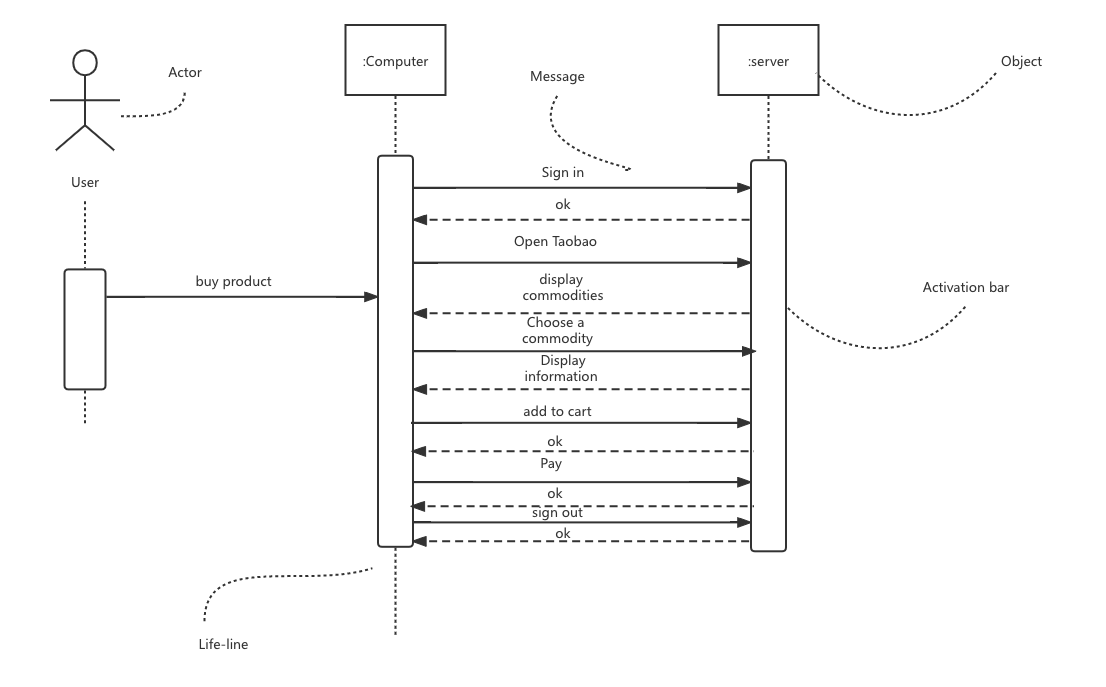
\includegraphics[width = 12cm]{picture/Sequence diagram.png}
\caption{The caption of this figure(Sequence diagram)}
\end{figure}
\end{document}